\section{Фактор-пространство}
Факторизирането е познато от други области като линейната алгебра и теория на групите, където разглеждаме множество елементи като един под действието на някакво изображение. По подобен начин ще разглеждаме и фактор-пространствата в топологията.

В геометричната интерпретация на топологията, факторизацията има смисъл на деформация и "залепване" на краищата.

\begin{example}
    Ако разгледаме квадрат и факторизираме като разглеждаме следните обекти като еквивалентни (ще покажем защо използваме точно тази дума по-долу в текста):

    \begin{itemize}
        \item Четирите ъгъла на квадрата
        \item Две по две успоредните страни
        \item Вътрешността на квадрата
    \end{itemize}

    Така полученото факторизиране всъщност е хомеоморфно на тор.
    \begin{figure}[H]
        \centering
        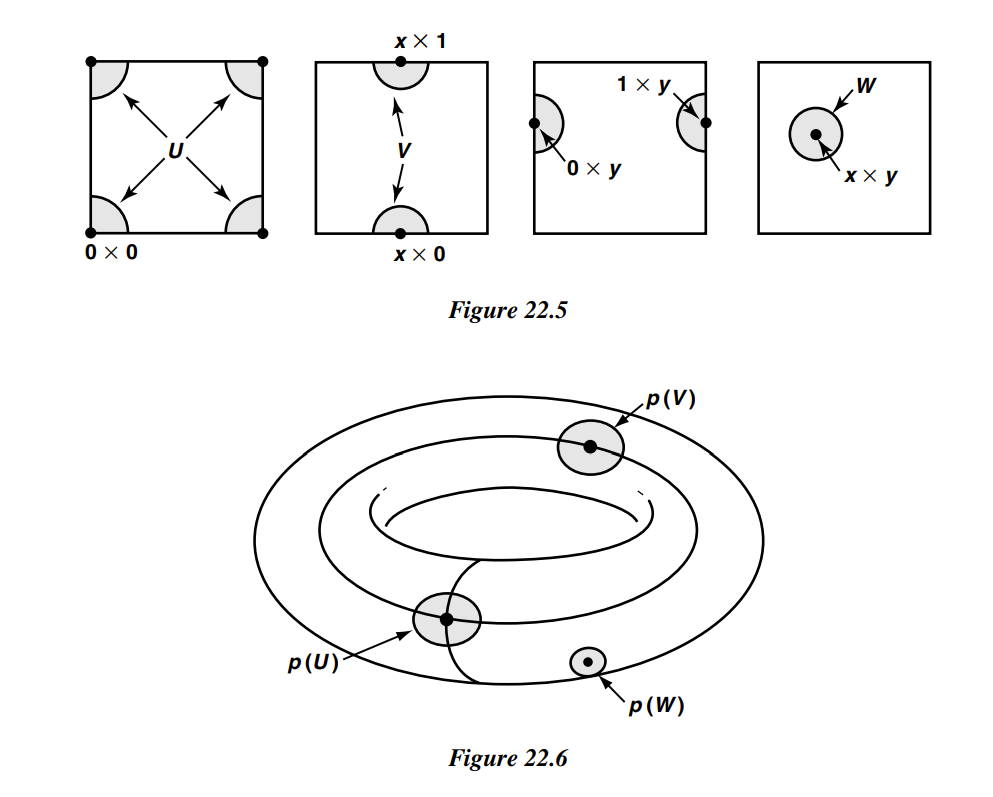
\includegraphics[width=\textwidth]{resources/torus.png}
        \caption{Визуално представяне на факторизацията (взето от \cite[стр.~140]{munkrestopology})}
    \end{figure}
\end{example}

\subsection{Факторно изображение}
\begin{definition}
    Нека $X, Y$ са топологични пространства.
    
    $p: X \to Y$. $p$ е факторно изображение $\bydef$ p е сюрекция и $\forall U \in Y$ - отворено множество: $p^{-1}(U)$ е отворено множество в $X$.
\end{definition}
\begin{notation}
    В тази секция употребяваме факторно (изборажение) като превод на "quotient map" или "strong continuity".
\end{notation}
\begin{definition}
    Нека $X$ е топологично пространство.
    
    $C \subseteq X$ е наситено(спрямо сюрективно изображение $p: X\to Y$) $\bydef$ $\forall y \in Y:\; p^{-1}(\{y\}) \cap C \neq \emptyset \rightarrow p^{-1}(\{y\}) \subseteq C$  .
\end{definition}
\begin{notation}
    Когато е ясно от контекста ще пропускаме "спрямо сюрективно изображение \dots".
\end{notation}
Иначе казано, $C$ е наситено точно тогава когато има такова подмножество на $U \subseteq Y$, че $p^{-1}(U) = C$.

Значи можем еквивалентно да дефинираме факторно изображение чрез наситени множества по следния начин:
\begin{proposition}
    $p: X \to Y$ е факторно изображение $\iff$ $p$ е непрекъснато изображение и изобразява наситените отворени множества на $X$ в отворени множества на $Y$.
\end{proposition}

Лесно може да се съобрази, че:
\begin{proposition}
    Нека $X, Y$ са топологични пространства.

    $p: X \to Y$ е сюрективно непрекъснато отворено/затворено изображение $\Rightarrow$ $p$ е факторно изображение.
\end{proposition}
\begin{remark}
    Това е достатъчно, но не е необходимо условие, т.е. има факторни изображения, които не са нито отворени, нито затворени.
\end{remark}
\begin{proof}
    Нека разглеждаме $\pi_1: \R \to \R$. Нека $A$ е подпространство на $\R \times \R$, т.ч.:
    \begin{equation}
        A = \{\langle x, y \rangle \mid x \geq 0 \lor y=0\}
    \end{equation}
    Нека $q : A \to \R$ дефинирано като рестрикцията на $\pi_1$ върху $A$.

    Тогава твърдим, че $q$ не е нито отворено, нито затворено изображение.

    \begin{itemize}
        \item[(не е отворено)] Търсим такова отворено множество $X \subseteq A$, че $q(X)$ не е отворено в стандартната топология на $\R$.
        
        Нека $X = [0; 1) \times \{0\}$. Тогава:
        \begin{equation}
            q(X) = [0; 1)
        \end{equation}
        Но това не е отворено множество $\R$.

        \item[(не е затворено)] Търсим такова затворено множество $X \subseteq A$, че $q(X)$ не е затворено в стандартната топология на $\R$.
        
        Нека $X = [0; 1) \times \{0\}$. Тогава:
        \begin{equation}
            q(X) = [0; 1)
        \end{equation}
        Но това не е затворено множество $\R$.
    \end{itemize}
    Значи можем да използваме един и същи контрапример за двата случая понеже интервалът $[0; 1)$ не е нито отворен, нито затворен.

    Не можем да изразим като крайно/безкрайно обединение и сечение на отворени интервали - няма как да "затворим" отляво интервала.
    \begin{equation}
        [0; 1) = \{0\} \cup (0; 1)
    \end{equation}
    Защото $\{0\}$ не е отворено множество.

    Допълнението му също не е отворено множество:
    \begin{equation}
        \overline{[0; 1)} = (-\infty; 0) \cup [1; \infty) = \bigcup_{n \in \N} (-n;0) \cup \{1\} \cup \bigcup_{n\in\N} (1+n;\infty)
    \end{equation}
    Защото $\{1\}$ не е отворено множество.
\end{proof}

\subsection{Фактор-топология дефинирана от изображение}
\begin{definition}
    Нека $X$ е топологично пространство, $A$ е произволно множество, $p: X \to A$ e сюрективно изображение.

    Тогава най-малката топология $\mathcal T$ над $A$, т.ч. $p$ е факторно изображение, се нарича Фактор-топология породенa от $p$.

    \begin{equation}
        \mathcal T = \{U \subseteq A \mid p^{-1}(U) \in \mathcal T_X\}
    \end{equation}
\end{definition}
Лесно се проверява, че е топология - при съмнение \cite[стр.~138]{munkrestopology}.

\begin{example}
    Нека $x \in \R$ е произволно и $A = \{a, b, c\}$ и $p: \R \to A$ дефинирано по следния начин:
    \begin{equation}
        p(y) = \begin{cases}
            a &, y > x\\
            b &, y < x\\
            c &, y = x
        \end{cases}
    \end{equation}

    Визуално топологията изглежда по следния начин:
    \begin{figure}[H]
        \centering
        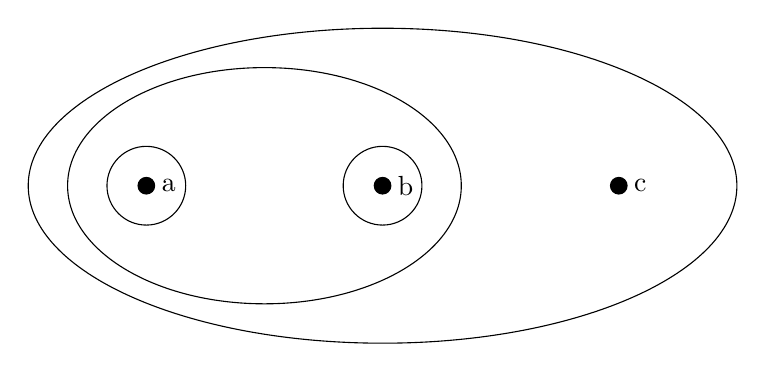
\begin{tikzpicture}
            \filldraw (-3, 0) circle (3pt) node [xshift = 2pt, anchor=west]{a};
            \filldraw (0, 0) circle (3pt) node [xshift = 2pt, anchor=west]{b};
            \filldraw (3, 0) circle (3pt) node [xshift = 2pt, anchor=west]{c};

            \draw (-3, 0) circle (0.5);
            \draw (0, 0) circle (0.5);
            % \draw (3, 0) circle (0.5);
            \draw (-1.5, 0) ellipse (2.5 and 1.5);
            \draw (0, 0) ellipse (4.5 and 2);
        \end{tikzpicture}
        \caption{Визуално представяне на топологията породена от $p$}
    \end{figure}
    
    \begin{remark}
        Забелязваме, че $c$ е елемент единствено на цялото множество - това се дължи на факта, че не можем да произведем полузатворен интервал с край $x$ - от вида $(v; x]$ или $[x; u)$.
    \end{remark}
    
    \begin{remark}
        Също полученото фактор-пространство не е Хаудосрфово.

        $a$ и $c$ не могат да бъдат отделени една от друга, защото $a$ е елемент на $\set{a}, \set{a, b}, A$, доката $c$ е елемент само на $A$. Няма околности, които да са непресичащи се.
    \end{remark}
\end{example}

\subsubsection{Композиция}
Лесно се проверява, че композицията запазва силната непрекъснатост благодарение на следния факт:
\begin{equation}
    p^{-1}(q^{-1}(x)) = (q \circ p)^{-1}(x)
\end{equation}
\begin{proposition}
    Нека $X_1, X_2, X_3$ са топологични пространства, $p_i: X_i \to X_{i+1}$ е факторно изображение за $i \in \{1, 2\}$.

    Тогава $p_1 \circ p_2 : X_1 \to X_3$ е факторно изображение.
\end{proposition}

\subsubsection{Произведение}
Декартовото произведение не винаги запазва силната непрекъснатост.
\begin{proof}
    Конструкция е.
    \cite[стр.~143]{munkrestopology}
\end{proof}

\subsection{Фактор-пространство дефинирано от релация на еквивалентност}
\subsubsection{Припомняне от теория на множествата}
\begin{definition}
    Нека $X$ е множество, а $\sim$ релация над $X$.

    $\sim$ е релация на еквивалентност $\bydef$ $\sim$ е рефлексивна, симетрична и транзитивна.
\end{definition}
\begin{definition}
    Нека $X$ е множество, а $\sim$ релация на еквивалентност над $X$. Клас на еквивалентност породен от $x \in X$ наричаме множество от всички елементи еквивалентни на $x$:
    \begin{eqnarray}
        [x] \overset{def}{=} \{y \in X \mid x \sim y \}
    \end{eqnarray}
\end{definition}

\begin{definition}
    Нека $X$ е множество, а $\sim$ релация на еквивалентност над $X$. $X$ факторизирано по $\sim$ наричаме фамилия от множества съставена от всички класове на еквивалентност:
    \begin{eqnarray}
        X/_\sim = \left\{[x] \mid x \in X\right\}
    \end{eqnarray}
\end{definition}

\begin{fact}
    Лесно се проверява, че два класа или съвпадат, или са непресичащи се:
    \begin{eqnarray}
        [x] \cap [y] = \begin{cases}
            [x] = [y] &, x \sim y\\
            \emptyset &, x \not\sim y
        \end{cases}
    \end{eqnarray}
\end{fact}

\begin{corollary}
    $X/_\sim$ е разбиване на $X$.
\end{corollary}
\begin{corollary}
    $X/_\sim$ поражда естествено сюрективно изображение $p: X \to X/_\sim,\; x \mapsto [x]$.
\end{corollary}

\subsubsection{Фактор-пространство}
\begin{definition}
    Нека $X$ е множество, $\sim$ е релация на еквивалентност над $X$, с естествено влагане $p: X \to X/_\sim$. С топологията породена от $p$, $X/_\sim$ се нарича фактор-пространство.
\end{definition}
\begin{proposition}
    Двете дефиниции за фактор-пространство са еквивалентни.
\end{proposition}
\begin{fact}
    Относно естественото включване, изображенията в двете посоки изглеждат по следния начин:

    От множеството към фактор-множеството:
    \begin{equation}
        p(X) = p(\{x_1, x_2, \dots, x_n, \dots\}) = \{[x_1], [x_2], \dots, [x_n], \dots\} = U
    \end{equation}

    От фактор-множеството към множеството:
    \begin{equation}
        p(U) = p(\{[x_1], [x_2], \dots, [x_n], \dots\}) = \bigcup_{[x] \in U} [x]
    \end{equation}
\end{fact}

\subsubsection{Относно подпространства}
\begin{theorem}
    Нека $X, Y$ са топологични пространства, $p: X \to Y$ е факторно изображение, $A \subseteq X$ е наситено подмножество. 

    Нека $q = p\mid_A, q: A \to p(A)$.
    \begin{itemize}
        \item Ако $A$ е отворено/затворено $\Rightarrow$ $q$ е факторно
        \item Ако $p$ е отворено/затворено изображение $\Rightarrow$ $q$ е факторно
    \end{itemize}
\end{theorem}
\begin{proof}
    \cite[стр.~140]{munkrestopology}.
\end{proof}

\subsection{Непрекъснати функции над фактор-пространство}

Подобно на \thref{th:sum-continuous} ще се интересуваме от това кога една функция е непрекъсната по отношение на това къде е дефинирана или нейните стойности.

Съответната на \thref{th:sum-continuous} по отношение на фактор-пространства е следната:
\begin{theorem}\label{th:factor-continuous}
    Нека $X, Y, Z$ са топологични пространства, $p: X \to Y$ е факторно изображение и $g: X \to Z$ е изображение, т.ч.
    \begin{equation}
        \exists z \in Z,\ \forall y \in Y:\; g(p^{-1}(\{y\})) = z
    \end{equation}
    т.е. $g$ е константа над всички множества от вида $p^{-1}(\{y\})$.

    Тогава $g$ поражда функция $f: Y \to Z,\ f \circ p = g$.
    \begin{itemize}
        \item $f$ е непрекъсната $\iff$ $g$ е непрекъсната
        \item $f$ е факторно $\iff$ $g$ е факторно
    \end{itemize}

    \begin{figure}[H]
        \centering
        \begin{tikzpicture}[
        node distance=3cm,
        auto
        ] 
           \node[state] (X) {$X$}; 
           \node[state] (Y) [below of = X] {$Y$}; 
           \node[state] (Z) [right of = Y]  {$Z$};
            \path[->] 
            (X) edge  node {$p$} (Y)
                edge  node {$g$} (Z)
            ;
            \path[->, dashed]
            (Y) edge node {$f$} (Z)
            ;
        \end{tikzpicture}
        \caption{Диаграмата е комутативна по формулировката на теоремата}
    \end{figure}
\end{theorem}
\begin{proof}
    \cite[стр.~142]{munkrestopology}.
\end{proof}
\begin{corollary}
    Нека $g: X \to Z$ е сюрективно непрекъснато изображение и $X^*$ е такова, че:
    \begin{equation}
        X^* = \{g^{-1}(\{z\}) \mid z \in Z\}
    \end{equation}
    $X^*$ е фактор-пространство породено от подходяща функция $p$.

    Тогава по \thref{th:factor-continuous} знаем, че има породена биективна\footnotemark  функция $f: X^* \to Z$, която е хомеоморфизъм, т.с.т.к. $g$ е факторно.  
    \footnotetext{праобразът (като множество) на дадено $z \in Z$ е напълно достатъчно, за да се опрелени еднозначно}.
\end{corollary}
\begin{proof}
    \cite[стр.~142-143]{munkrestopology}.
\end{proof}

\subsection{Примери}
Допълнителни примери за факторни изображения и фактор-пространства по релация на еквивалентност. Вж. \cite[стр.~144-145]{munkrestopology}.
\begin{example}
    Нека $X$ е топологично пространство и $A \subset X$, тогава $id_X\mid_A$ е факторно изображение.
\end{example}
\begin{example}
    Дефинираме релация $\sim$ над $\R^2$:
    \begin{equation}
        \langle x_0, y_0 \rangle \sim \langle x_1, y_1 \rangle \bydef x_0 + y_0^2 = x_1 + y_1 ^2
    \end{equation}
    Очевидно е релация на еквивалентност основавайки се на факта, че $=$ е релация на еквивалентност.

    Да разгледаме няколко класа на еквивалентност:
    \begin{equation}
        [\langle 0, 0 \rangle] = \{ \langle -x^2, x \rangle \mid x \in \R_0^+\}
    \end{equation}
    Това е графиката на $x^2$ завъртяна с $\frac{\pi}{2}$.
    \begin{equation}
        [\langle 0, 1 \rangle] = \{ \langle -x^2 + 1, x \rangle \mid x \in \R_0^+\}
    \end{equation}
    Това е графиката на $x^2 - 1$ завъртяна с $\frac{\pi}{2}$.

    Забелязваме, че:
    \begin{equation}
        a\in \R:\; [\langle 0, a \rangle] = \{ \langle -x^2 + a^2, x \rangle \mid x \in \R_0^+\}
    \end{equation}

    Да се опитаме да варираме първата координата:
    \begin{equation}
        [\langle 1, 0 \rangle] = \{ \langle -x^2 + 1, x \rangle \mid x \in \R_0^+\}
    \end{equation}
    \begin{equation}
        [\langle 2, 0 \rangle] = \{ \langle -x^2 + 2, x \rangle \mid x \in \R_0^+\}
    \end{equation}
    \begin{equation}
        a\in \R:\; [\langle a, 0 \rangle] = \{ \langle -x^2 + a, x \rangle \mid x \in \R_0^+\}
    \end{equation}
    \begin{equation}
        [\langle 1, 1 \rangle] = \{ \langle -x^2 + 2, x \rangle \mid x \in \R_0^+\}
    \end{equation}
    \begin{equation}
        [\langle 2, 1 \rangle] = \{ \langle -x^2 + 3, x \rangle \mid x \in \R_0^+\}
    \end{equation}
    \begin{equation}
        a \in \R:\; [\langle a, 1 \rangle] = \{ \langle -x^2 + a + 1, x \rangle \mid x \in \R_0^+\}
    \end{equation}
    \begin{equation}
        a \in \R:\; [\langle a, 2 \rangle] = \{ \langle -x^2 + a + 4, x \rangle \mid x \in \R_0^+\}
    \end{equation}
    Забелязваме вече шаблона, затова твърдим:
    \begin{equation}
        a, b \in \R:\; [\langle a, b \rangle] = \{ \langle -x^2 + a + b^2, x \rangle \mid x \in \R_0^+\}
    \end{equation}
\end{example}